\documentclass{source/Report}



\major{电子科学与技术}
\name{朱炳昊}
\title{NA Project}
\stuid{3220105656}
\college{信息与电子工程学院}
\date{\today}
\lab{西2-213}
\course{数值分析方法}
\instructor{余官定}
\grades{}
\expname{稀疏矩阵特征值}
\exptype{大作业报告}
\partner{无}

\begin{document}
\makecover
\makeheader
\tableofcontents
\section{背景介绍}
在实际的工程和科学应用中,我们经常会遇到大规模的数据集,这些数据通常以矩阵的形式呈现。许多情况下,这些矩阵主要由零元素构成,只有少部分非零元素,我们称这种矩阵为“稀疏矩阵”。在诸如社交网络分析、图像处理、自然语言处理、有限元分析、物理学模拟等多个领域,我们都会遇到稀疏矩阵。由于这些领域的数据通常具有高维度,但又由于各种原因,矩阵中的数据元素只有极小一部分是非零的,因此,如何处理和利用这些稀疏矩阵变得非常重要。

作为一名正在学习数值分析方法课程的学生,我对这个问题有着浓厚的兴趣。我知道,计算和理解稀疏矩阵的特征值是一个具有挑战性的问题。然而,存在一些专门的数值计算方法,如Power Method、QR 算法和 Arnoldi迭代算法,可以帮助我们解决这个问题。

在本次期末大作业中,我打算深入研究这些算法,并将它们应用在普通矩阵和高维稀疏矩阵上,比较他们在不同类型矩阵上的性能。我相信,通过这项研究,我将能够更深入地理解稀疏矩阵的重要性,以及特征值计算方法的应用。
\section{设计思路}
\subsection{设计目的}
本研究的主要目的是探索和理解数值计算方法在处理稀疏矩阵特征值问题上的应用和性能表现。具体来说,设计目标可分为以下几点:

(1)深入理解Power Method、QR算法和Arnoldi迭代算法的工作原理和应用场景,以及如何将它们应用于稀疏矩阵的特征值计算。

(2)比较这些算法在普通矩阵和高维稀疏矩阵上的性能表现,包括计算速度、精度和稳定性等方面。

(3)深入理解稀疏矩阵在不同领域的应用,以及特征值计算在这些应用中的重要性。

(4)建立一个能够处理大规模稀疏矩阵特征值问题的计算模型,以展示这些数值计算方法在实际工程和科学应用中的效用。

通过完成这些目标,我们希望能够为稀疏矩阵特征值的计算提供一种有效的数值计算工具,同时也为理解和应用稀疏矩阵提供一种新的视角和理论支持。
\subsection{设计流程}
\begin{itemize}
  \item \textbf{Import necessary libraries:} 首先,我们需要导入开发过程中需要用到的库。
  \item \textbf{Define functions:} 接着,我们定义了一些数学计算函数,包括'sparse\_sym\_matrix'、'power\_method'、'qr\_iteration'、'arnoldi\_iteration1'和'arnoldi\_iteration2'。这些函数分别用于生成稀疏矩阵、实现幂法、QR迭代法和Arnoldi迭代法。
  \item \textbf{Define MainWindow class:} 然后,我们定义了主窗口类'MainWindow',该类主要用于构建用户界面和处理用户操作。
  \item \textbf{Define methods in MainWindow class:} 在'MainWindow'类中,我们定义了一些方法,包括'run\_code'和'open\_readme'。'run\_code'方法用于获取用户输入,调用相应的函数执行计算,然后显示结果。'open\_readme'方法用于打开GitHub上的说明文档。
  \item \textbf{Create QApplication object and MainWindow object:} 最后,我们创建了'QApplication'对象和'MainWindow'对象,并显示GUI窗口。
\end{itemize}

使用Graphviz绘制的流程图如下所示:
\begin{figure}[H]
  \centering
  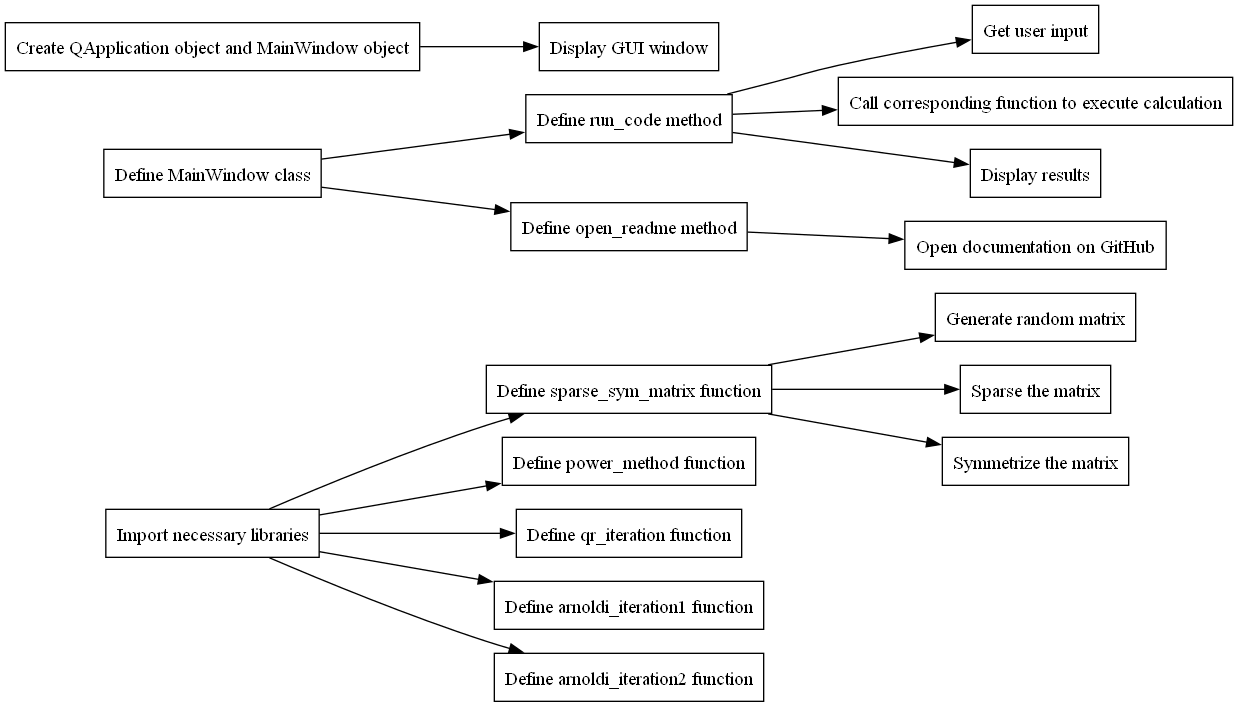
\includegraphics[width = 1\textwidth]{lct}
  \caption{设计流程图}
\end{figure}

\subsection{设计环境}
运行环境为 Python 3.11.5,以下为运行python文件所需调用的库:
\begin{itemize}
  \item \textbf{numpy:} Python科学计算的核心库,提供了高性能的多维数组对象及相关工具。
  \item \textbf{scipy:} 基于numpy的一种高级计算库,提供了许多有用的数学算法和函数。
  \item \textbf{PyQt5:} Python编写的GUI框架,用于创建桌面应用程序。
  \item \textbf{sys:} Python内置库,提供了访问与Python解释器紧密相关的变量和函数的途径。
  \item \textbf{webbrowser:} Python内置库,提供了一个简单的接口,用于在Web浏览器中显示文档或打开URL。
\end{itemize}

\section{算法描述}
\subsection{稀疏矩阵的密度}
矩阵$A\in \mathbb{R} ^{m\times n}$,其密度定义为非零元素数量与总元素数量的比值:
\[density = \dfrac{num(a_{ij}\neq 0)}{mn},\]\par
其中,$a_{ij}$为矩阵 $A$ 第 $i$ 行第 $j$ 列的元素。

\subsection{Power Method}
Power Method 是一种求解矩阵最大(绝对值)特征值和对应特征向量的算法。它的基本思想是,给定一个可对角化的矩阵 $A$ 和一个非零向量 $x$ ,重复计算 $y = Ax$ 和 $x = y / ||y||$ ,直到 $x$ 收敛到一个单位向量。这个单位向量就是 $A$ 的一个特征向量,而 $A$ 对这个特征向量的作用就是乘以一个标量,这个标量就是 $A$ 的最大特征值。幂迭代法的优点是简单易实现,缺点是收敛速度较慢,且只能求解最大特征值和特征向量。
\begin{algorithm}[H]
  \caption{The Power Method}
  \begin{algorithmic}[1]
    \Require dimension $n$; matrix $A$; vector $x$; tolerance $TOL$; maximum number of iterations $N$.
    \Ensure approximate eigenvalue $\mu$; approximate eigenvector $x$ (with $\|x\|_{\infty} = 1$) or a message that the maximum number of iterations was exceeded.
    \State Set $k = 1$.
    \State Find the smallest integer $p \leq n$ such that $|x_p| = \|x\|_\infty$
    \State Set $x = x/x_p$
    \While{$k \leq N$}
    \State Set $y = Ax$
    \State Set $\mu = y_p$
    \State Find the smallest integer $p \leq n$ such that $|y_p| = \|y\|_\infty$
    \If{$y_p = 0$}
    \State OUTPUT ('Eigenvector'); STOP
    \EndIf
    \State Set $ERR = \|x-(y/y_p)\|_{\infty}$
    \State Set $x=y/y_p$
    \If{$ERR < TOL$}
    \State OUTPUT ($\mu$, x); STOP
    \EndIf
    \State Set $k = k + 1$
    \EndWhile
    \State OUTPUT ('Maximum number of iterations exceeded'); STOP
  \end{algorithmic}
\end{algorithm}

\subsection{Givens变换}
又叫吉文斯旋转(Givens Rotation),一般用来数值求解矩阵的QR分解。数值求解矩阵的QR分解的基本思想是将原目标矩阵 A 左乘一系列正规正交变换矩阵 $H_1,H_2,...,H_n$ 后得到一个上三角矩阵,该上三角矩阵即为 $R$ 矩阵, $H_n...H_2H_1A=HA=Q^{-1}A=R$ ,其中 H 矩阵的逆矩阵即为 Q 矩阵。

吉文斯旋转,顾名思义,就是将原本的列向量保持长度不变旋转一个角度,使之平行于坐标轴即其中一个元素为零。一般使用吉文斯方法是逐列进行行变换的,从第一列开始,从下往上将对角线以下的元素都变为零,每次变换仅将一个元素变为零,例如找到一个变换矩阵 \[G=\begin{pmatrix} g_1 & g_2 \\ g_3 & g_4 \\ \end{pmatrix} \]

使得 \[\begin{pmatrix} g_1 & g_2 & \cdots & 0 \\ g_3 & g_4 & \cdots & 0 \\ \vdots & \vdots & \ddots & \vdots \\ 0 & 0 & \cdots & 1 \end{pmatrix}\begin{pmatrix} a_{1,1} & a_{1,2} & \cdots & a_{1,n} \\ a_{2,1} & a_{2,2} & \cdots & a_{2,n} \\ \vdots & \vdots & \ddots & \vdots \\ 0 & a_{m,2} & \cdots & a_{m,n} \end{pmatrix}=\begin{pmatrix} b_{1,1} & b_{1,2} & \cdots & b_{1,n} \\ 0 & b_{2,2} & \cdots & b_{2,n} \\ \vdots & \vdots & \ddots & \vdots \\ 0 & b_{m,2} & \cdots & b_{m,n} \end{pmatrix}\]

即\[ \begin{pmatrix} g_1 & g_2 \\ g_3 & g_4 \\ \end{pmatrix} \begin{pmatrix} a_1 \\ a_2 \\ \end{pmatrix}= \begin{pmatrix} \sqrt{a_1^2+a_2^2} \\ 0 \\ \end{pmatrix}= \begin{pmatrix} b_1 \\ 0 \\ \end{pmatrix} \]

可以发现满足该需求的变换矩阵为吉文斯变换矩阵 \[G=\begin{pmatrix} c & s \\ -s & c \\ \end{pmatrix} \]

其中 $$c=cos\theta=\frac{a_1}{\sqrt{a_1^2+a_2^2}},s=sin\theta=\frac{a_2}{\sqrt{a_1^2+a_2^2}}$$

这里一般使用的吉文斯变换矩阵的c和s的位置是固定的。

\begin{algorithm}
  \caption{Givens Reduction}
  \begin{algorithmic}[1]
    \Require matrix $A$ of size $n \times n$
    \Ensure orthogonal matrix $Q$ and upper triangular matrix $R$ such that $A = QR$
    \State Set $R = A$
    \State Set $G\_list = []$
    \For{$j = 0$ to $n - 1$}
    \For{$i = j + 1$ to $n - 1$}
    \If{$R[i][j] = 0$}
    \State continue
    \EndIf
    \State Set $a = R[j][j]$
    \State Set $b = R[i][j]$
    \State Set $base = \sqrt{a^2 + b^2}$
    \State Set $c = a / base$
    \State Set $s = b / base$
    \State Set $G = I_n$
    \State Set $G[j][j] = c$
    \State Set $G[i][j] = -s$
    \State Set $G[j][i] = s$
    \State Set $G[i][i] = c$
    \State Set $R = G R$
    \State Append $G$ to $G\_list$
    \EndFor
    \EndFor
  \end{algorithmic}
\end{algorithm}
\begin{algorithm}
  \caption{Givens Reduction(cont'd)}
  \begin{algorithmic}[1]
    \State Set $R = R[0:n]$
    \State Set $Q\_prime = I_n$
    \For{each $G$ in $G\_list$}
    \State Set $Q\_prime = G Q\_prime$
    \EndFor
    \State Set $Q = Q\_prime[0:n]^T$
    \State Return $Q, R$
  \end{algorithmic}
\end{algorithm}

\subsection{QR算法}
$Q R$ 算法的核心思路是利用矩阵的 $Q R$ 分解, 迭代构造一系列矩阵并最终收敛为上三角矩阵, 从而计算特征值。具体而言, 矩阵 $A \in \mathbb{R}^{n \times n}$ 可以通过 $\mathrm{QR}$ 分解得到 $A=Q R$, 其中 $Q$为正交矩阵, $R$ 为上三角阵。通过构建矩阵序列 $A_{k+1}=R_k Q_k=Q_k^{\top} A_k Q_k$, 可以得到矩阵序列 $\left\{A_k\right\}$ ,其中每一个矩阵 $A_k$ 都与矩阵 $A$ 相似,即具有相同的特征值。假设特征值各不相同且降序排列, 可以证明矩阵 $A_k$ 中下三角的元素满足 $\left|a_{i j}^{(k)}\right|=\mathcal{O}\left(\left|\lambda_i / \lambda_j\right|^k\right), i>j$ 。因此, 当 $\mathrm{k}$趋于无穷时, $A_k$ 收敛为上三角矩阵, 此时的对角线元素即为特征值。

有三种方法可以用于实现 $Q R$ 分解:Gram-Schmidt 正交化过程,Householder 变换和 Givens 变换。这里我们采用了Givens变换法来进行QR分解,下方给出了QR迭代的伪代码。

\begin{algorithm}
  \caption{QR Iteration}
  \begin{algorithmic}[1]
    \Require matrix $A$ of size $n \times n$; number of eigenvalues $k$
    \Ensure a list of $k$ largest eigenvalues of $A$ in absolute value
    \State Set $M = A$
    \For{$i = 1$ to $1000$}
    \State Set $Q, R = \text{Givens\_reduce}(M)$
    \State Set $M = R Q$
    \EndFor
    \State Set $M_1 = Q R$
    \State Set $eigenvalues = []$
    \For{$i = 0$ to $n - 1$}
    \State Append $M_1[i][i]$ to $eigenvalues$
    \EndFor
    \State Sort $eigenvalues$ by absolute value in descending order
    \State Return $eigenvalues[0:k]$
  \end{algorithmic}
\end{algorithm}

\subsection{Arnoldi迭代}

Arnoldi 迭代算法的核心思路是将矩阵投影到低维 Krylov 子空间, 从而将矩阵约化为上 Hessenberg 矩阵, 从而计算其特征值。通过低维 Krylov 子空间, Arnoldi 迭代并不直接利用矩阵本身, 而是利用矩阵向量乘积, 从而减小处理高维矩阵时的复杂度。具体而言, 对于给定的矩阵 $A \in \mathbb{R}^{n \times n}$ 和向量 $b \in \mathbb{R}^n$, Krylov 序列为向量集合 $\left\{b, A b, A^2 b, A^3 b, \cdots\right\}$ 。M 维Krylov 子空间定义为长度为 $m$ 的 Krylov 序列张成的空间(可以把序列中的向量理解为基向量):
$$
  \mathcal{K}_m(A, b) \triangleq \operatorname{span}\left\{a, A b, A^2 b, \cdots, A^{m-1} b\right\}
$$

Arnoldi 迭代期望将矩阵分解为 $A=Q H Q^{\top}$ ,其中 $H$ 为上 Hessenberg 矩阵, $Q$ 为正交矩阵。将矩阵 $Q$ 表示为列向量形式 $Q=\left[q_1\left|q_2\right| \cdots \mid q_n\right]$, 并矩阵分解形式转换为 $A Q=Q H$,其第 $m$ 列的结果可以表示为:
$$
  A q_m=h_{1 m} q_1+h_{2 m} q_2+\cdots+h_{m+1, m} q_{m+1},
$$

其中, $h_{i, m}=0, i>m+1$ 。利用上式可以推导向量 $q_{m+1}$ 的递归形式:
$$
  q_{m+1}=\frac{A q_m-\sum_{i=1}^m h_{i, m} q_i}{h_{m+1, m}}
$$

不难发现, 实际上这与 Gram-Schmidt 求正交基的方法非常类似, $q_m$ 就是 Krylov 子空间的正交基。通过求解的正交矩阵 $Q$, 我们可以计算 Hessenberg 矩阵 $H=Q^{\top} A Q$ 。由于 $H$ 与 $A$ 相似, 可以利用已有算法计算 $H$ 的特征值从而得到 $A$ 的特征值。

值得注意的是, 对于高维矩阵我们往往只关注其一部分的特征值, 比如只考虑前 $k \ll n$列。此时, 可以将矩阵分解简化为矩阵分解为 $A Q_k=Q_{k+1} \tilde{H}_k$, 其中 $Q_k=\left[q_1\left|q_2\right| \cdots \mid q_k\right]$, $\tilde{H}_k=\left[\begin{array}{ccccc}h_{11} & h_{12} & \cdots & & h_{1, k} \\ h_{21} & h_{22} & \cdots & & h_{2, k} \\ 0 & h_{32} & \ddots & h_{k-1, k-1} & \vdots \\ & 0 & \ddots & h_{k, k-1} & h_{k, k} \\ & & & 0 & h_{k+1, k}\end{array}\right]$


\begin{algorithm}
  \caption{Algorithm 1 Arnoldi Iteration}
  \begin{algorithmic}[1]
    \State choose $b$ arbitrarily, then $q_1 = b/\|b\|_2$
    \For{$m = 1,2,\dots,k$}
    \State $v=Aq_m$
    \For{$j = 1,2,\dots,m$}
    \State $h_{jm} = v_j - q_j^Tv$
    \State $v=v-h_{jm}q_j$
    \EndFor
    \State $h_{m+1,m} = \|v_{m+1}\|_2$
    \State $q_{m+1} = v_{m+1}/h_{m+1,m}$
    \EndFor
  \end{algorithmic}
\end{algorithm}




\section{应用展示与代码呈现}
\subsection{UI界面}
首先展示一下我们的UI界面,如下图所示:
\begin{figure}[H]
  \centering
  
\includegraphics[width = 0.6\textwidth]{ui}
  \caption{UI界面}
\end{figure}

分为了四个界面,分别对应4道题的解答。
同时在界面下方有两个按钮:
\begin{figure}[H]
  \centering
  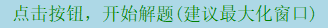
\includegraphics[width = 0.65\textwidth]{jt}
  \caption{解题按钮}
\end{figure}

解题按钮用于开启题目的计算,点击后稍等几秒,会在各个界面输出相应的计算结果,由于初始化界面较小,建议将界面最大化来清晰地比对结果,如下图所示:
\begin{figure}[H]
  \centering
  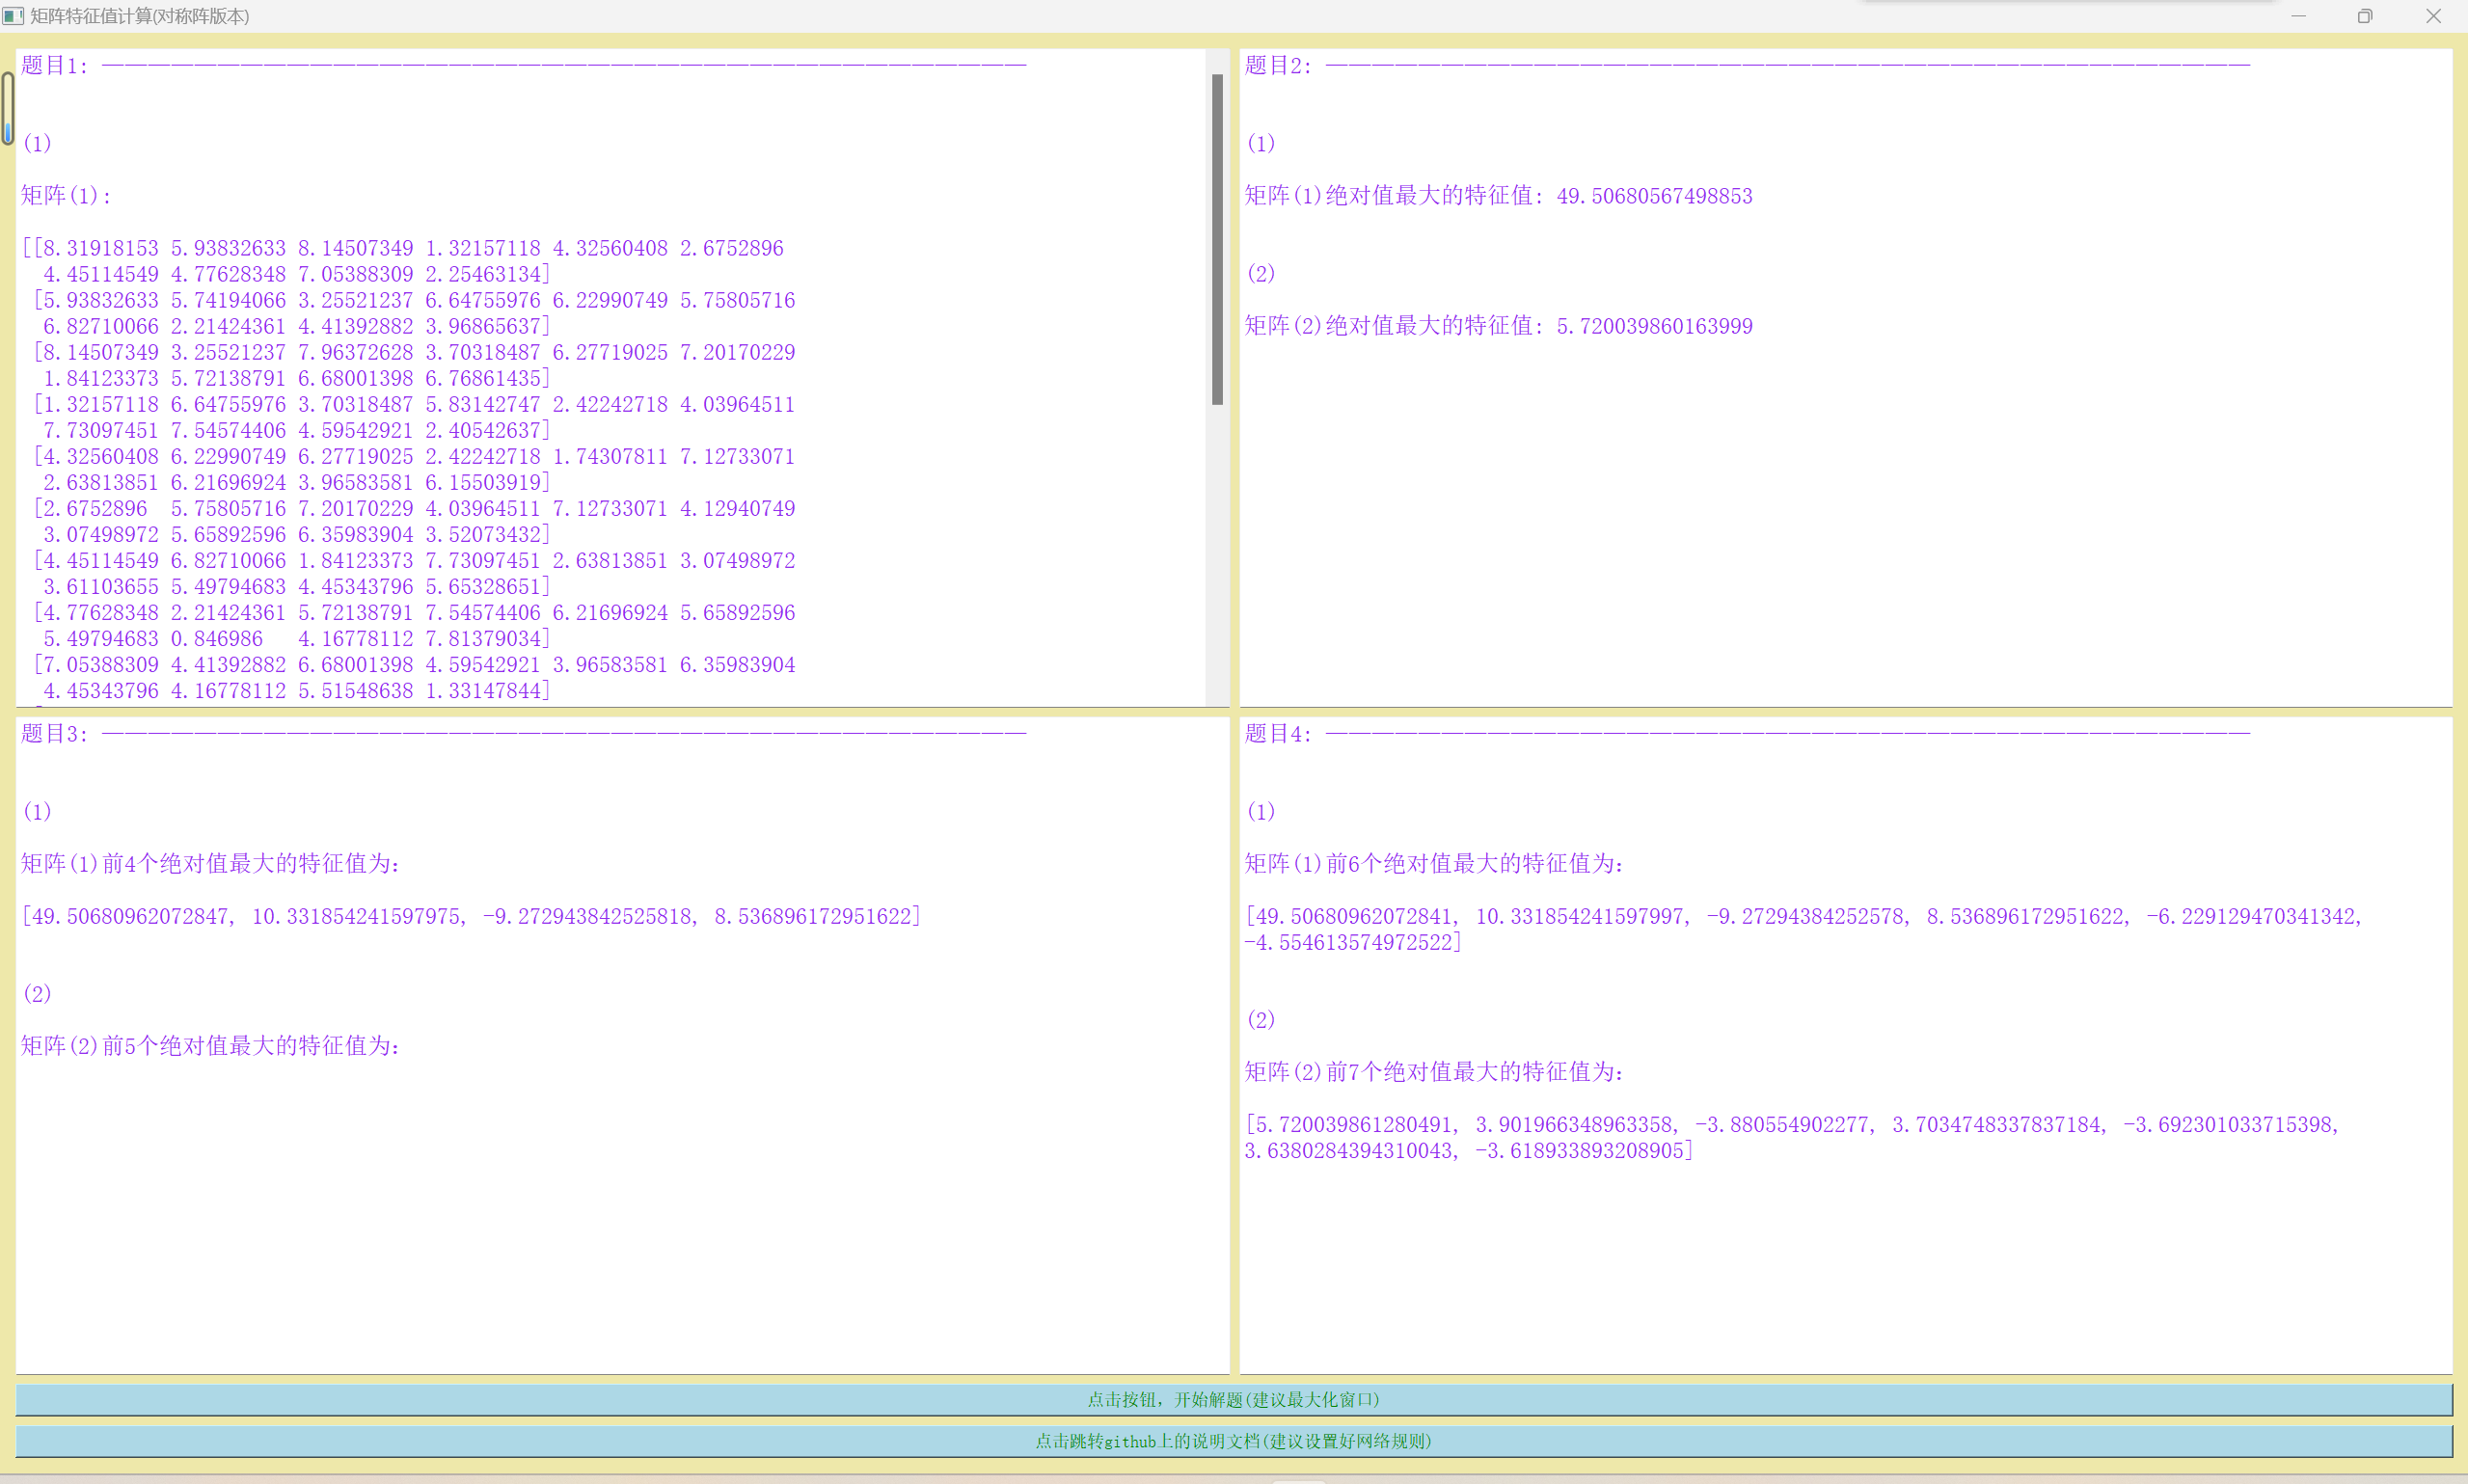
\includegraphics[width = 0.65\textwidth]{js}
  \caption{计算结果}
\end{figure}

以及说明按钮:
\begin{figure}[H]
  \centering
  
\includegraphics[width = 0.7\textwidth]{sm}
  \caption{说明按钮}
\end{figure}

点击说明按钮,会在默认浏览器中打开本项目的GitHub网站上的说明文档(github有时候需要科学上网,所以请设置好自己的代理规则),如下图所示:
\begin{figure}[H]
  \centering
  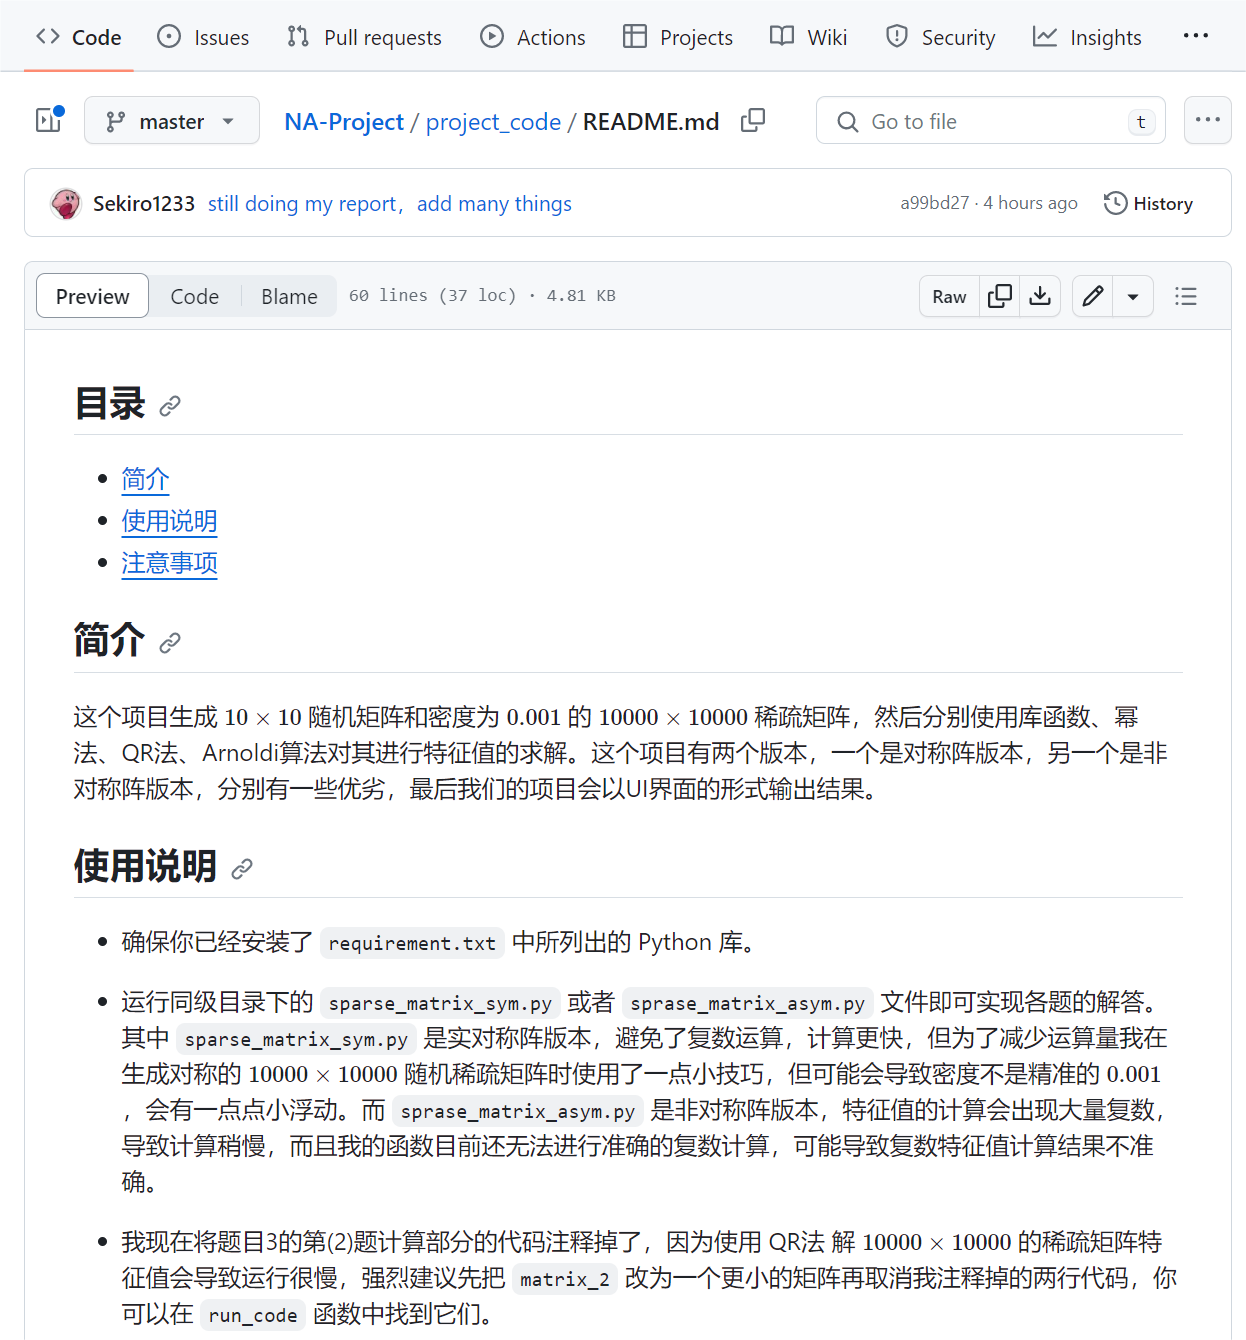
\includegraphics[width = 0.7\textwidth]{mk}
  \caption{说明文档}
\end{figure}

\subsection{题目1}
生成随机矩阵

(1)生成一个 $10\times10$ 维度的随机矩阵。

(2)生成一个 $10000\times 10000$ 维度且密度为 $0.001$ 的随机稀疏矩阵,并统计矩阵中非零元素数量。

(3)利用库函数计算(1)和(2)中矩阵的特征值。

\subsection*{(1)}
我选择直接使用$'np.random.rand(10, 10) * 10'$来生成元素大小在0到10之间的随机矩阵:
\begin{figure}[H]
  \centering
  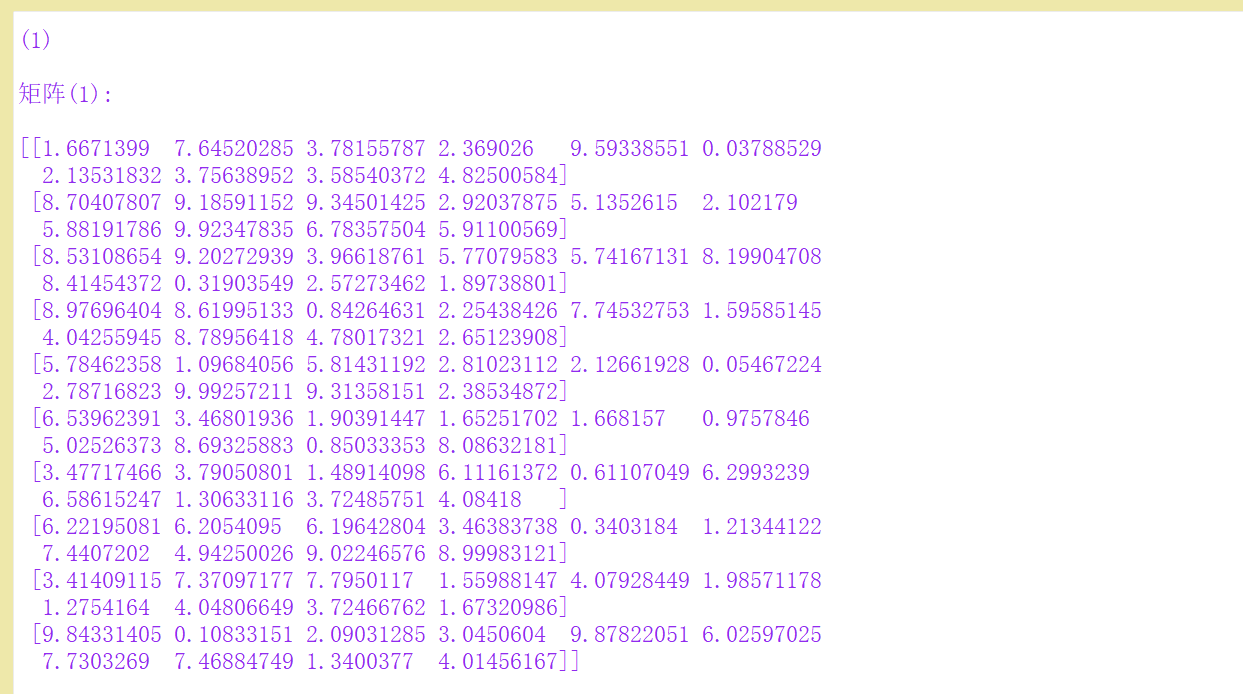
\includegraphics[width = 0.7\textwidth]{p11a}
  \caption{生成随机矩阵}
\end{figure}

当然这样生成出来的矩阵是一个不对称的矩阵,计算特征值的时候有很大概率是复数,所以我又使用$'matrix = (matrix + matrix.T) / 2'$生成一个对称矩阵:
\begin{figure}[H]
  \centering
  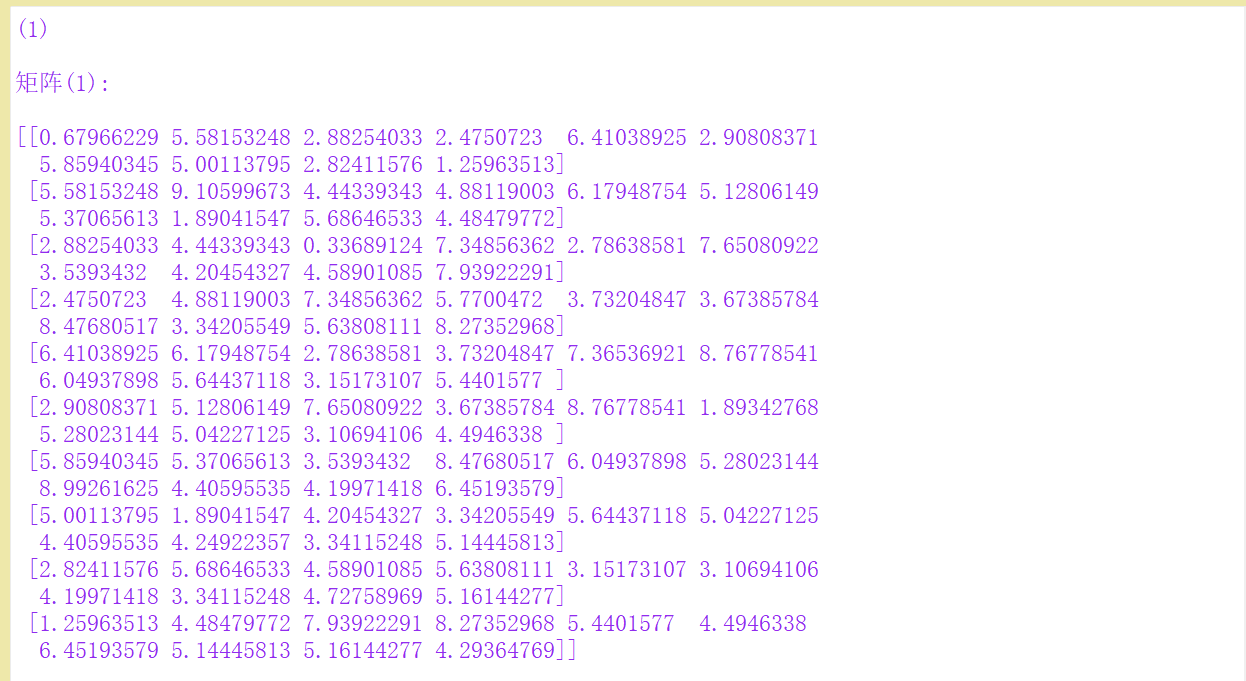
\includegraphics[width = 0.7\textwidth]{p11}
  \caption{生成随机对称矩阵}
\end{figure}

这样子生成出来的矩阵就是一个对称矩阵了,可以直接计算特征值,而且因为是实对称矩阵,特征值不会出现复数。

\subsection*{(2)}
我使用$'matrix = random(10000, 10000, density=0.001) * 10'$来生成题目要求的随机稀疏矩阵,计算元非零素数量可以得到:
\begin{figure}[H]
  \centering
  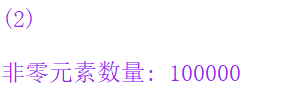
\includegraphics[width = 0.3\textwidth]{p12a}
  \caption{随机稀疏矩阵非零元素数量}
\end{figure}

然后我首先使用$'np.triu_indices'$生成上三角矩阵的所有索引,然后从中随机选择一部分。使用$'np.random.choice'$的$'replace=False'$选项来确保所有选择的索引对都是唯一的。由于是在上三角矩阵中选择元素,然后再将其反射到下三角矩阵,因此,元素总数应该是 $n * (n + 1) / 2$。

\begin{lstlisting}[language = Python, title = {生成随机对称稀疏矩阵}]
def sparse_sym_matrix(n, density):
    num_elements = int(n * (n + 1) * density / 2)
    indices = np.triu_indices(n)
    available_positions = len(indices[0])
    positions = np.random.choice(available_positions, size=num_elements, replace=False)
    row = indices[0][positions]
    col = indices[1][positions]
    data = np.random.rand(num_elements)
    upper_tri = sparse.coo_matrix((data, (row, col)), shape=(n, n))
    lower_tri = sparse.coo_matrix((data, (col, row)), shape=(n, n))
    return upper_tri + lower_tri
\end{lstlisting}

这种算法的好处在于避免了对很大的矩阵进行直接的操作运算,生成速度很快,缺点在于由于生成元素具有随机性,所以生成的矩阵的密度可能会与预期有一点点不符。

\subsection*{(3)}
接下来是使用库函数来计算我们生成矩阵的特征值,这里我使用了$'np.linalg.eigvals'$和$'scipy.sparse.linalg.eigs'$来计算特征值,结果如下:

\begin{figure}[htbp]
  \centering
  \subfigure[非对称阵特征值]{
    \label{fig:subfig:a}
    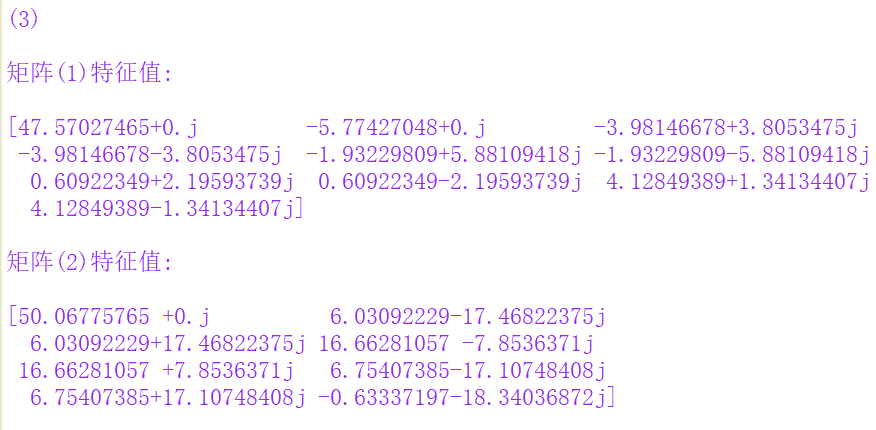
\includegraphics[width=0.45\textwidth]{p13a.png}}
  \subfigure[对称阵特征值]{
    \label{fig:subfig:b}
    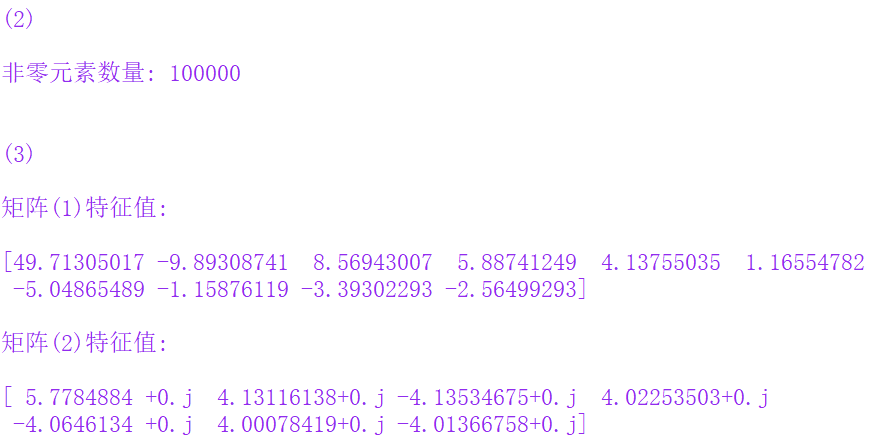
\includegraphics[width=0.45\textwidth]{p123.png}}
  \label{fig:subfig}
  \caption{库函数特征值计算结果}
\end{figure}

可以看到,对于非对称矩阵,库函数计算出来的特征值有可能是复数,而对于对称矩阵,库函数计算出来的特征值都是实数,与预期相同。

\subsection{题目2}
(1)利用 Power Method 计算题目 1(1)中矩阵的绝对值最大的特征值。

(2)利用 Power Method 计算题目 1(2)中稀疏矩阵的绝对值最大的特征值。\\ \par

根据算法部分写出的伪代码,我们可以得到以下代码:

\begin{lstlisting}[language = Python, title = {Power Method 代码}]
# 实现power method
def power_method(matrix, tol, max_iter):
    k = 1
    n = matrix.shape[0]
    x = np.random.rand(n)
    x = x / np.linalg.norm(x, np.inf)  # 归一化,使得||x||∞ = 1
    while k <= max_iter:
        p = np.argmin(np.abs(x))
        x = x / x[p]
        y = matrix @ x
        p = np.argmin(np.abs(y))
        if y[p] == 0:
            return "y[p] == 0", x
        mu = y[p]
        err = np.linalg.norm(x - y / y[p], np.inf)
        x = y / y[p]
        if err < tol:
            return mu, x
        k += 1
    return "The maximum number of iterations exceeded"
\end{lstlisting}

求解即可得到:

\begin{figure}[htbp]
  \centering
  \subfigure[非对称阵特征值]{
    \label{fig:subfig:a}
    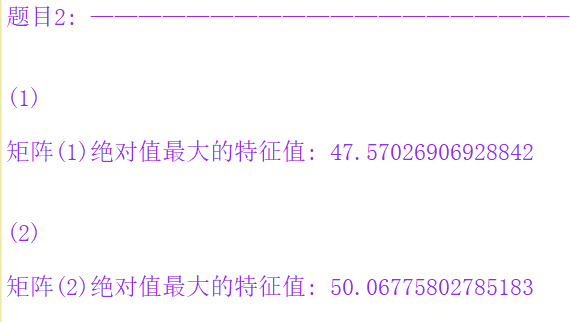
\includegraphics[width=0.45\textwidth]{p2a.png}}
  \subfigure[对称阵特征值]{
    \label{fig:subfig:b}
    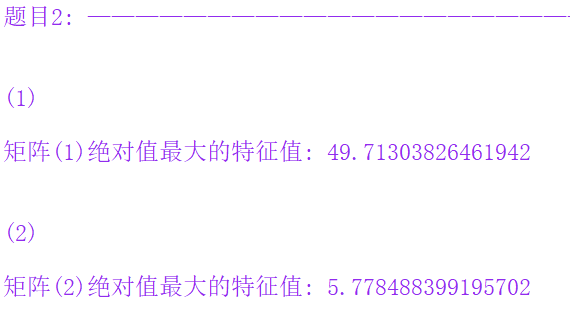
\includegraphics[width=0.45\textwidth]{p2.png}}
  \label{fig:subfig}
  \caption{Power Method 特征值计算结果}
\end{figure}

对比库函数计算结果,我们可以发现幂法的计算结果到达预期。需要注意的(2)有时候可能遇到$y[p] == 0$的情况,会输出$'y[p] == 0'$,这种情况就需要重新计算了。

\subsection{题目3}

(1)利用 QR 算法计算题目 1(1)中矩阵的前 4 个绝对值最大的特征值。

(2)利用 QR 算法计算题目 1(2)中稀疏矩阵的前 5 个绝对值最大的特征值。\\ \par

\subsection*{(1)}
我们使用基于Givens变换的QR分解法,再利用QR迭代求解特征值,其中QR迭代代码如下:

\begin{lstlisting}[language = Python, title = {QR Iteration 代码}]
# 实现QR迭代求解特征值
def qr_iteration(matrix, k):
    n = matrix.shape[0]
    for i in range(1000):
        q, r = givens_reduce(matrix)
        matrix = np.dot(r, q)
    matrix_1 = np.dot(q, r)
    eigenvalues = []
    for i in range(n):
        eigenvalues.append(matrix_1[i, i])
        eigenvalues = sorted(eigenvalues, key=lambda x: abs(x), reverse=True)[:k]
    return eigenvalues
\end{lstlisting} 

计算题目1(1)随机矩阵特征值,我们得到:
\begin{figure}[htbp]
  \centering
  \subfigure[非对称阵特征值]{
    \label{fig:subfig:a}
    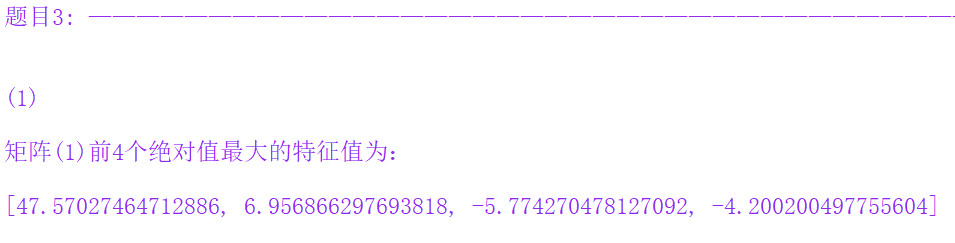
\includegraphics[width=0.75\textwidth]{p31a.png}}
  \subfigure[对称阵特征值]{
    \label{fig:subfig:b}
    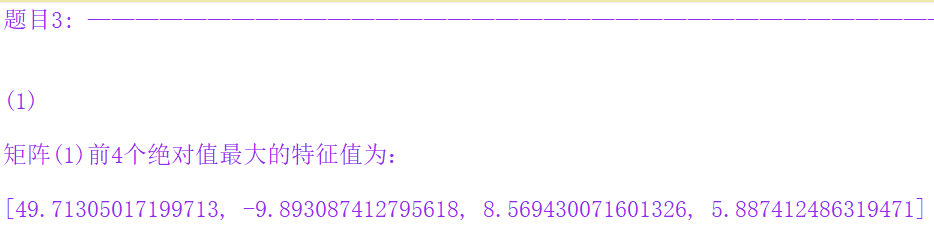
\includegraphics[width=0.75\textwidth]{p3.png}}
  \label{fig:subfig}
  \caption{QR 特征值计算结果}
\end{figure}

我们可以看到,非对称阵关于复数特征值的计算存在误差,但是对于对称阵,QR算法对于实数特征值计算出来的特征值与库函数计算结果相差很小。
\subsection*{(2)}

我们可以看到题目3(2)是没有输出的,因为我把输出与计算部分的函数注释掉了,因为使用python,加上我的QR算法可能存在的问题,导致计算$10000\times 10000$的稀疏矩阵特征值很慢,于是我这里选择用小一点的稀疏矩阵来测试,生成$100\times 100$且密度为$0.01$的稀疏矩阵,然后取消我代码中注释掉的部分,运行程序,得到结果如下:

\begin{figure}[htbp]
  \centering
  \subfigure[库函数特征值计算结果]{
    \label{fig:subfig:a}
    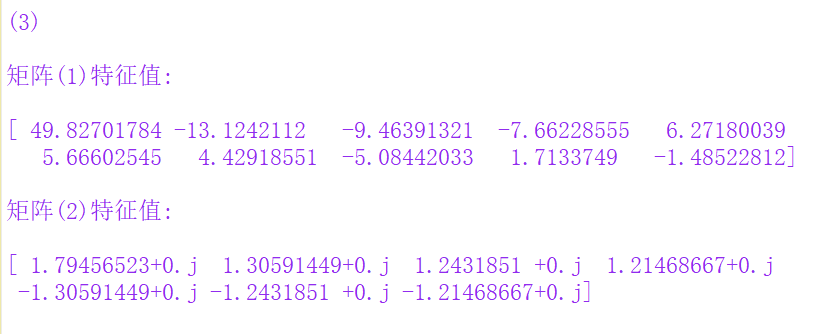
\includegraphics[width=0.75\textwidth]{one.png}}
  \subfigure[QR法特征值计算结果]{
    \label{fig:subfig:b}
    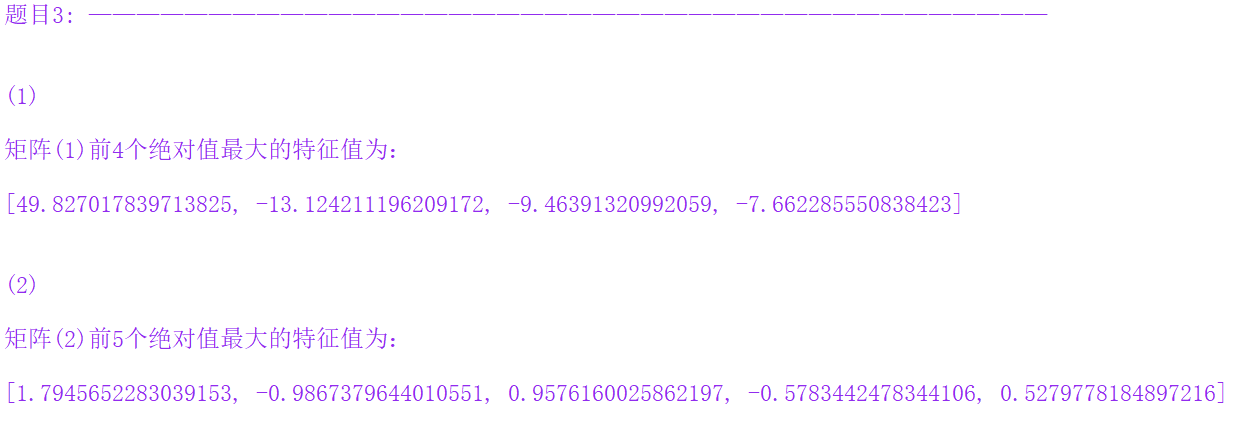
\includegraphics[width=0.75\textwidth]{two.png}}
  \label{fig:subfig}
  \caption{特征值计算结果}
\end{figure}

可以观察到对于稀疏矩阵,最大绝对值的特征值计算还是准确的,但随着继续计算余下的特征值,误差越来越大,而对于小的密集矩阵,计算结果就没有问题。

\subsection{题目4}

(1)利用 Arnoldi 迭代算法计算题目 1(1)中矩阵的前 6 个绝对值最大的特征值。

(2)利用 Arnoldi 迭代算法计算题目 1(2)中稀疏矩阵的前 7 个绝对值最大的特征值。\\ \par

我们先使用Arnoldi迭代得到矩阵H,然后对矩阵H使用QR迭代法求解特征值。对矩阵(1)使用Arnoldi算法时,由于迭代次数少,我们直接选10列来迭代,让计算结果更准确;而对于稀疏矩阵,我们选择一个较少的列来迭代(这里我们选择前30列,如果想让计算结果更准确可以选择更多的列数),增加迭代速度,同时也能得到较准确的结果:

\begin{figure}[H]
  \centering
  \subfigure[非对称阵特征值]{
    \label{fig:subfig:a}
    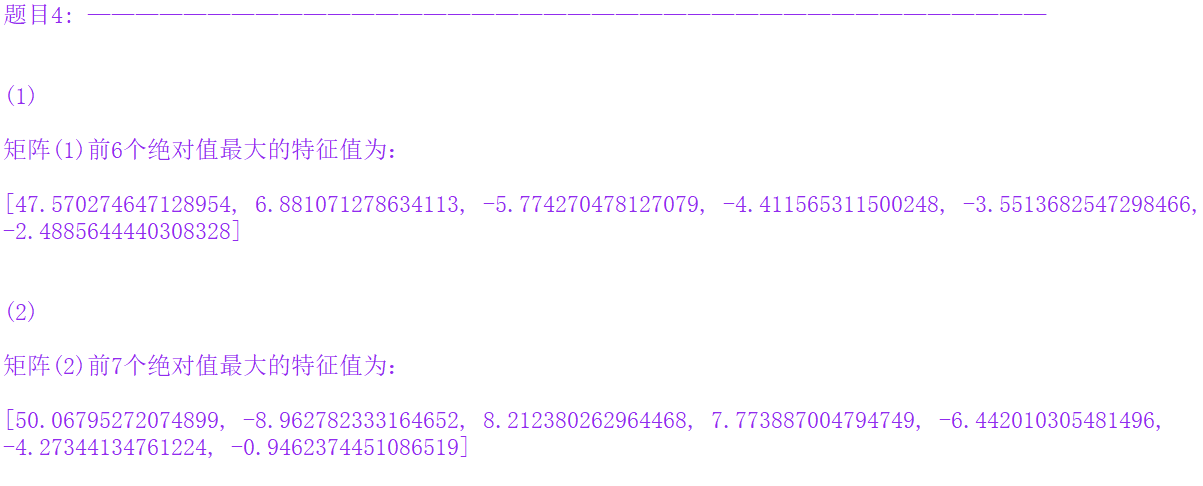
\includegraphics[width=0.75\textwidth]{p4a.png}}
  \subfigure[对称阵特征值]{
    \label{fig:subfig:b}
    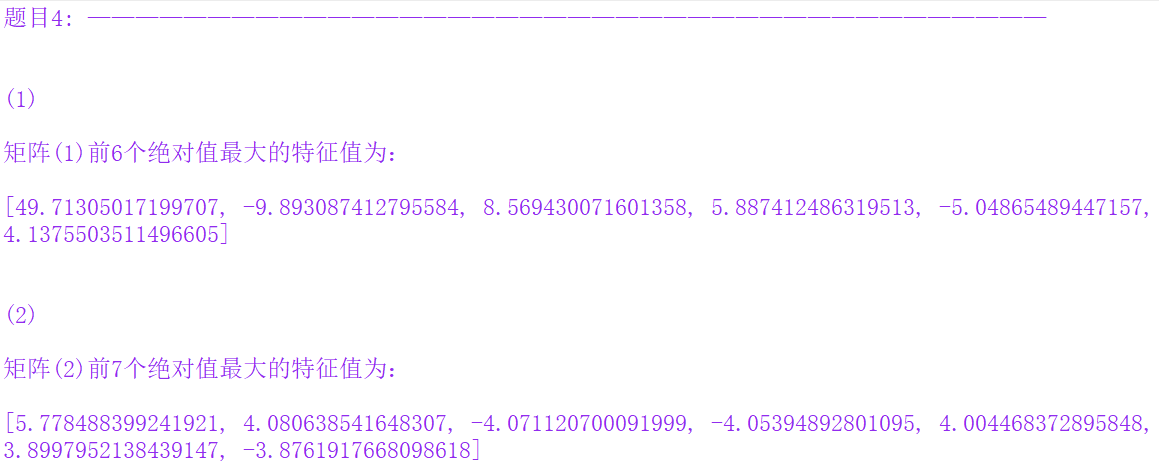
\includegraphics[width=0.75\textwidth]{p4.png}}
  \label{fig:subfig}
  \caption{Arnoldi迭代特征值计算结果}
\end{figure}

观察结果,我们可以发现对于密集矩阵,实数的特征值求解结果准确,但对于复数特征值求解存在误差;对于稀疏矩阵,我们可以看到,Arnoldi迭代法求解特征值的结果与QR迭代法求解特征值的结果相差很小,但是Arnoldi迭代法的计算速度要快很多。同样,因为只选取前k列($k<<n$),计算得到的最大值准确,越往后计算误差越大,可以适当增加k值来提升计算精度,但计算时间也会增加。



\section{时间复杂度分析}

\section{使用说明}

\section{总结与展望}


% \begin{table}[H]
%     \centering
%     \caption{雅可比迭代结果-4.1}
%     \begin{tabular}{cccc}
%     \toprule
%     $n$ & $x_1^{(n)}$ & $x_2^{(n)}$ & $x_3^{(n)}$ \\
%     \midrule
%     0 & 1.25000000 & -1.33333333 & 0.20000000 \\
%     1 & 1.63333333 & -0.85555556 & -0.11111111 \\
%     2 & 1.43611111 & -0.81759259 & -0.04740741 \\
%     \bottomrule
%     \end{tabular}
% \end{table}\par


% \lstinputlisting[
%     language = Python,
%     title = {最小二乘法线性拟合代码}
% ]{code/linear_ap.py}\par


%             \begin{lstlisting}[language = Verilog, title = {代码块测试(直接插入)}]
% module dffre (
%     d, en, r, clk, q
% );
%     parameter n = 1;
%     input en,r,clk;
%     input [n-1:0] d;
%     output [n-1:0] q;
%     reg [n-1:0] q;
%     always @(posedge clk) begin
%         if(r) q = {n{1'b0}};
%         else if(en) q = d;
%             else q = q;
%     end
% endmodule
%             \end{lstlisting}

%             \begin{figure}[H]
%                 \centering
%                 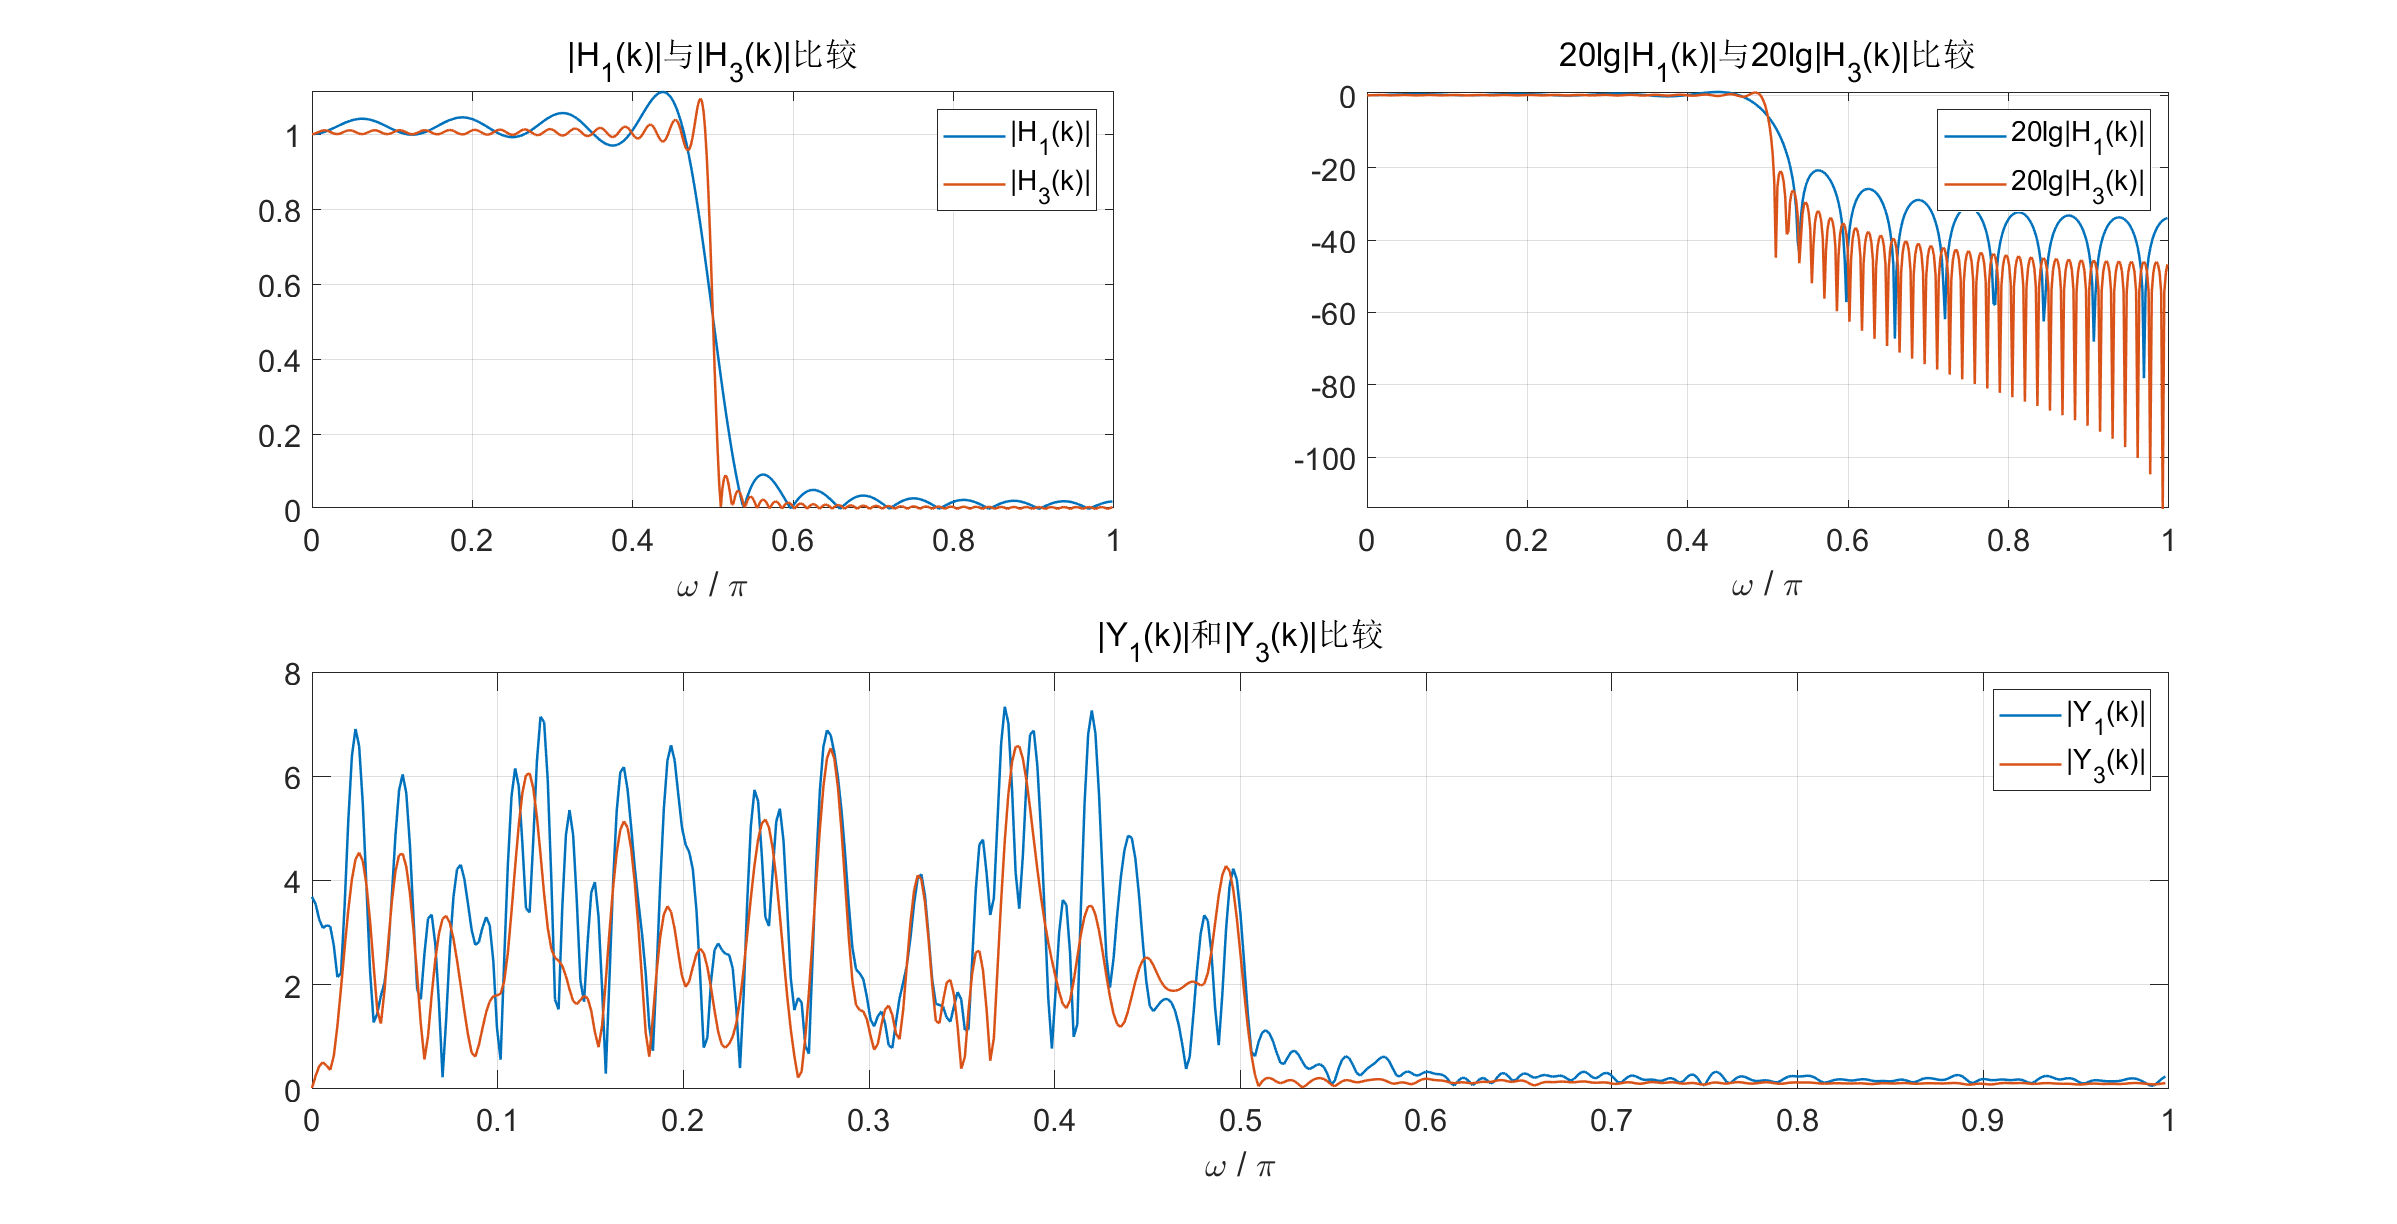
\includegraphics[width = 1\textwidth]{pic1}
%                 \caption{图片测试}
%             \end{figure}


% \section{}
%         \subsection{}
%         1\footnote{测试}2
%         \begin{table}[H]
%             \centering
%             \caption{表格测试}
%             \begin{tabular}{|c|c|c|c|c|c|c|c|c|}
%             \hline
%             state                 & ld & st & addr{[}31:11{]} == tag & valid & dirty & l2\_ack & write\_done & nextstate                   \\ \hline
%             \multirow{4}{*}{Idle} & 0  & 0  & -                      & -     & -     & -       & -           & Idle                        \\ \cline{2-9} 
%                                 & 0  & 1  & -                      & -     &       & -       & -           & \multirow{3}{*}{CompareTag} \\ \cline{2-8}
%                                 & 1  & 0  & -                      & -     &       & -       & -           &                             \\ \cline{2-8}
%                                 & 1  & 1  & -                      & -     &       & -       & -           &                             \\ \hline
%         \end{tabular}
%         \end{table}
\end{document}